\documentclass{beamer}
\geometry{papersize={12.8cm,7.6cm}}
% \documentclass[aspectratio=169]{beamer}

%----------------------------------------------------------------------------------------
%	PACKAGES & SETUP
%----------------------------------------------------------------------------------------
\usepackage{ragged2e}
\usepackage{etoolbox}

\usepackage[useregional]{datetime2}
\usepackage{graphicx,url}
\usepackage{hyperref}
\usepackage[utf8]{inputenc}
\usepackage[brazil]{babel}
\usepackage{booktabs}
\usepackage{amsmath}
\usepackage{xcolor}
\definecolor{lightblue}{RGB}{0,191,255}
\usepackage[textsize=tiny,backgroundcolor=lightblue,linecolor=lightblue]{todonotes}
\usepackage[bf,sf,footnotesize,indent,justification=centering]{caption}
\usepackage[caption=true,font=footnotesize]{subfig}
\usepackage{ textcomp }
\usepackage{color, colortbl}
% \definecolor{name}{system}{definition}
\definecolor{Gray}{gray}{0.9}
\definecolor{LightCyan}{rgb}{0.5,1,1}

\captionsetup[subfigure]{
    justification=centering,
    labelfont={bf,sf},
    textfont={bf,sf,footnotesize},
    singlelinecheck=off,justification=centering
}
\captionsetup[figure]{
    justification=centering,
    labelfont={bf,sf},
    textfont={bf,sf,footnotesize},
    singlelinecheck=off
}
\captionsetup[table]{
    justification=centering,
    labelfont={bf,sf},
    textfont={bf,sf,footnotesize},
    singlelinecheck=off,
    justification=centering
}

\mode<presentation> {
    \usetheme{Frankfurt}
    \usecolortheme{whale}
    \setbeamertemplate{navigation symbols}{}
    \setbeamertemplate{footline}[page number]
}

%----------------------------------------------------------------------------------------
%	PRESENTATION SLIDES
%----------------------------------------------------------------------------------------

\thispagestyle{empty}

\title[FEC with Ensembles of CNN and Smart Voting]{Facial Expressions Classification with Ensembles of
Convolutional Neural Networks and Smart Voting}

\author{Rodrigo C. Moraes \and Elloá B. Guedes \and Carlos Maurício S. Figueiredo}
\institute[UEA]
{
Universidade do Estado do Amazonas - UEA \\
Escola Superior de Tecnologia - EST \\
Laboratório de Sistemas Inteligentes - LSI \\
\bigskip
\textit{\{rcm.eng, ebgcosta, cfigueiredo\}@uea.edu.br}
}
\date{06 de Dezembro de 2019}
\apptocmd{\frame}{}{\justifying}{}

\begin{document}

\begin{frame}[label=firstframe]
    \titlepage
\end{frame}

\begin{frame}
    \frametitle{Sumário}
    \tableofcontents
\end{frame}

%------------------------------------------------
\section{Introdução}
%https://ibug.doc.ic.ac.uk/media/uploads/documents/EncycBiometrics-Pantic-FacExpRec-PROOF.pdf
A Classificação de Expressões Faciais é um processo executado por humanos e computadores que consiste em localizar faces em uma cena, extrair características faciais da região detectada, analisar alterações das características faciais como um sorriso ou um franzir de sobracelhas, e categorizar o resultado em uma expressão como felicidade ou raiva, por exemplo \cite{Pantic2009fea}.

Tecnologias que podem interpretar e responder de forma automática a expressões faciais já encontram uma grande variedade de aplicações, dada sua importância social. Exemplos disto, são sistemas de ensino que utilizam a expressão facial dos alunos como \textit{feedback}, teste da efetividade de fármacos anti-depressivos e detecção de fadiga de motoristas e pilotos \cite{Fasel2003}.

Graças a introdução de métodos de \textit{Machine Learning}, tem-se  avançado no campo de Classificação Automática de Expressões Faciais. Mais especificamente, métodos de \textit{Deep Learning} tem apresentado resultados bons nas tarefas que envolvem o uso de detecção de padrões e extração de características em imagens, nas mais variadas situações e contextos \cite{whitehill2013automatic}.

Paul Ekman e Friesen postularão seis emoções primárias que possuem cada uma conteúdo próprio e associação a uma única expressão facial. Estas emoções se monstram invariantes ao longo das diversas culturas humanas e são identificadas como felicidade, tristeza, medo, nojo, surpresa e raiva \cite{Ekman1971}.

O presente trabalho apresentou resultados equiparáveis ao da literatura na tarefa de Classificação Automática de Expressões Faciais nas expressões primárias, utilizando modificação não-trivial, votação mediada por um modelo inteligente, em \textit{Emsemble} de Redes Neurais Convolucionais.

%------------------------------------------------

%------------------------------------------------
\section{Base de dados}
A base de dados de expressões faciais utilizada para o desenvolvimento deste trabalho é denominada \emph{Facial Expression Recognition Challenge} (FER2013). Esta base contém $35.887$ imagens faciais em escala de cinza com dimensões de $48\times 48$ pixels, rotuladas de maneira supervisionada segundo uma das sete expressões faciais universais, conforme amostras ilustradas na Figura \ref{fig:samples}.

\begin{figure}[h!]
	\centering
  \captionof{figure}{Amostras de imagens faciais da base de dados FER2013.}
  \label{fig:samples}

	\begin{tabular}{@{}c@{}}
		\subfloat[Felicidade]{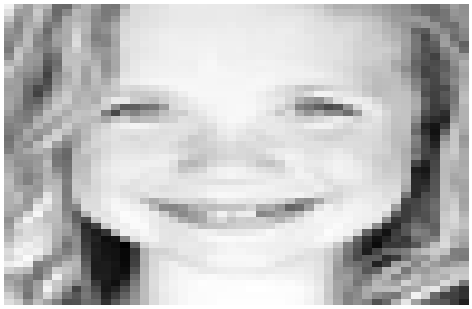
\includegraphics[width=0.15\linewidth]{images/sample_happy.png}}
		\subfloat[Nojo]{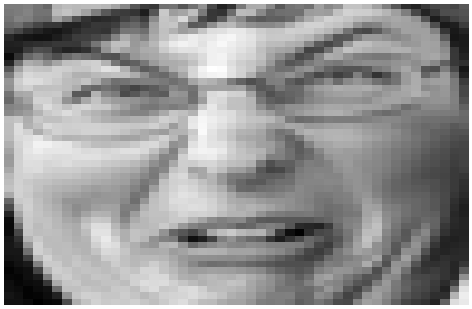
\includegraphics[width=0.15\linewidth]{images/sample_disgust.png}}
		\subfloat[Tristeza]{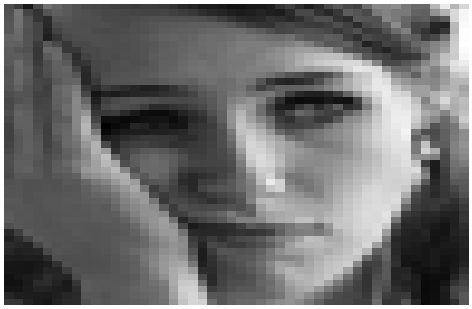
\includegraphics[width=0.15\linewidth]{images/sample_sad.png}}
	\end{tabular}

	\vspace{\floatsep}

  \begin{tabular}{@{}c@{}}
		\subfloat[Surpresa]{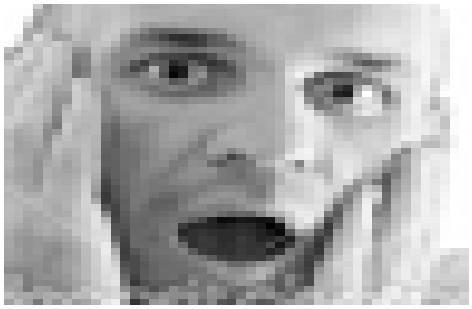
\includegraphics[width=0.15\linewidth]{images/sample_surprise.png}}
  	\subfloat[Medo]{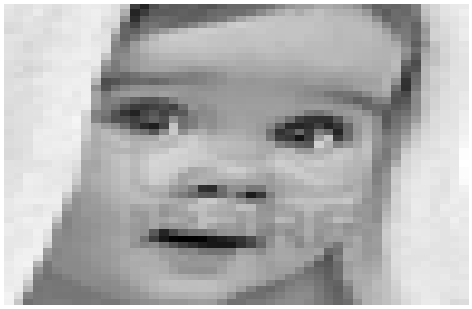
\includegraphics[width=0.15\linewidth]{images/sample_fear.png}}
  	\subfloat[Raiva]{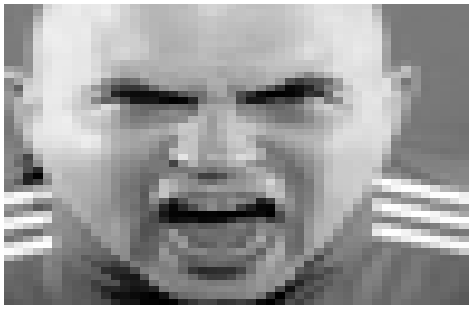
\includegraphics[width=0.15\linewidth]{images/sample_angry.png}}
    \subfloat[Neutro]{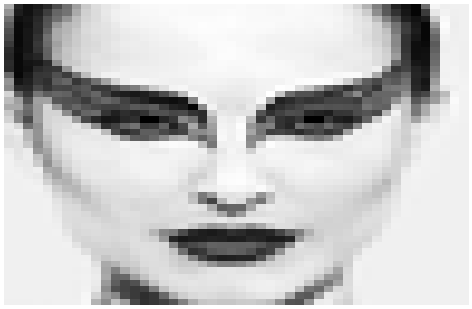
\includegraphics[width=0.15\linewidth]{images/sample_neutral.png}}
  \end{tabular}
\end{figure}

Conforme ilustra a Figura \ref{fig:samples}, é interessante notar algumas características particulares das imagens do FER2013 que ressaltam a relevância desta base de dados. Observa-se que, embora as faces estejam centralizadas nas imagens, elementos como cortes de cabelo, barba, óculos e até mesmo mãos encontram-se presentes, diminuindo a distância entre os exemplos contidos nesta base de dados e aqueles passíveis de ocorrência em um cenário realístico.

Os exemplos disponíveis na FER2013 se distribuem de maneira heterogênea perante as classes consideradas, conforme ilustra o gráfico da Figura \ref{fig:dataset}. O número de exemplos rotulado com a expressão ``nojo'', por exemplo, representam apenas $1.5\%$ do total de exemplos disponíveis. Estas características evidenciam o desbalanceamento do conjunto de dados considerado no tocante à quantidade de amostras por classe.

\begin{figure}[!htb]
    \centering
    \caption{Distribuição de imagens por tipo de expressão facial na base FER2013.}  \label{fig:dataset}
    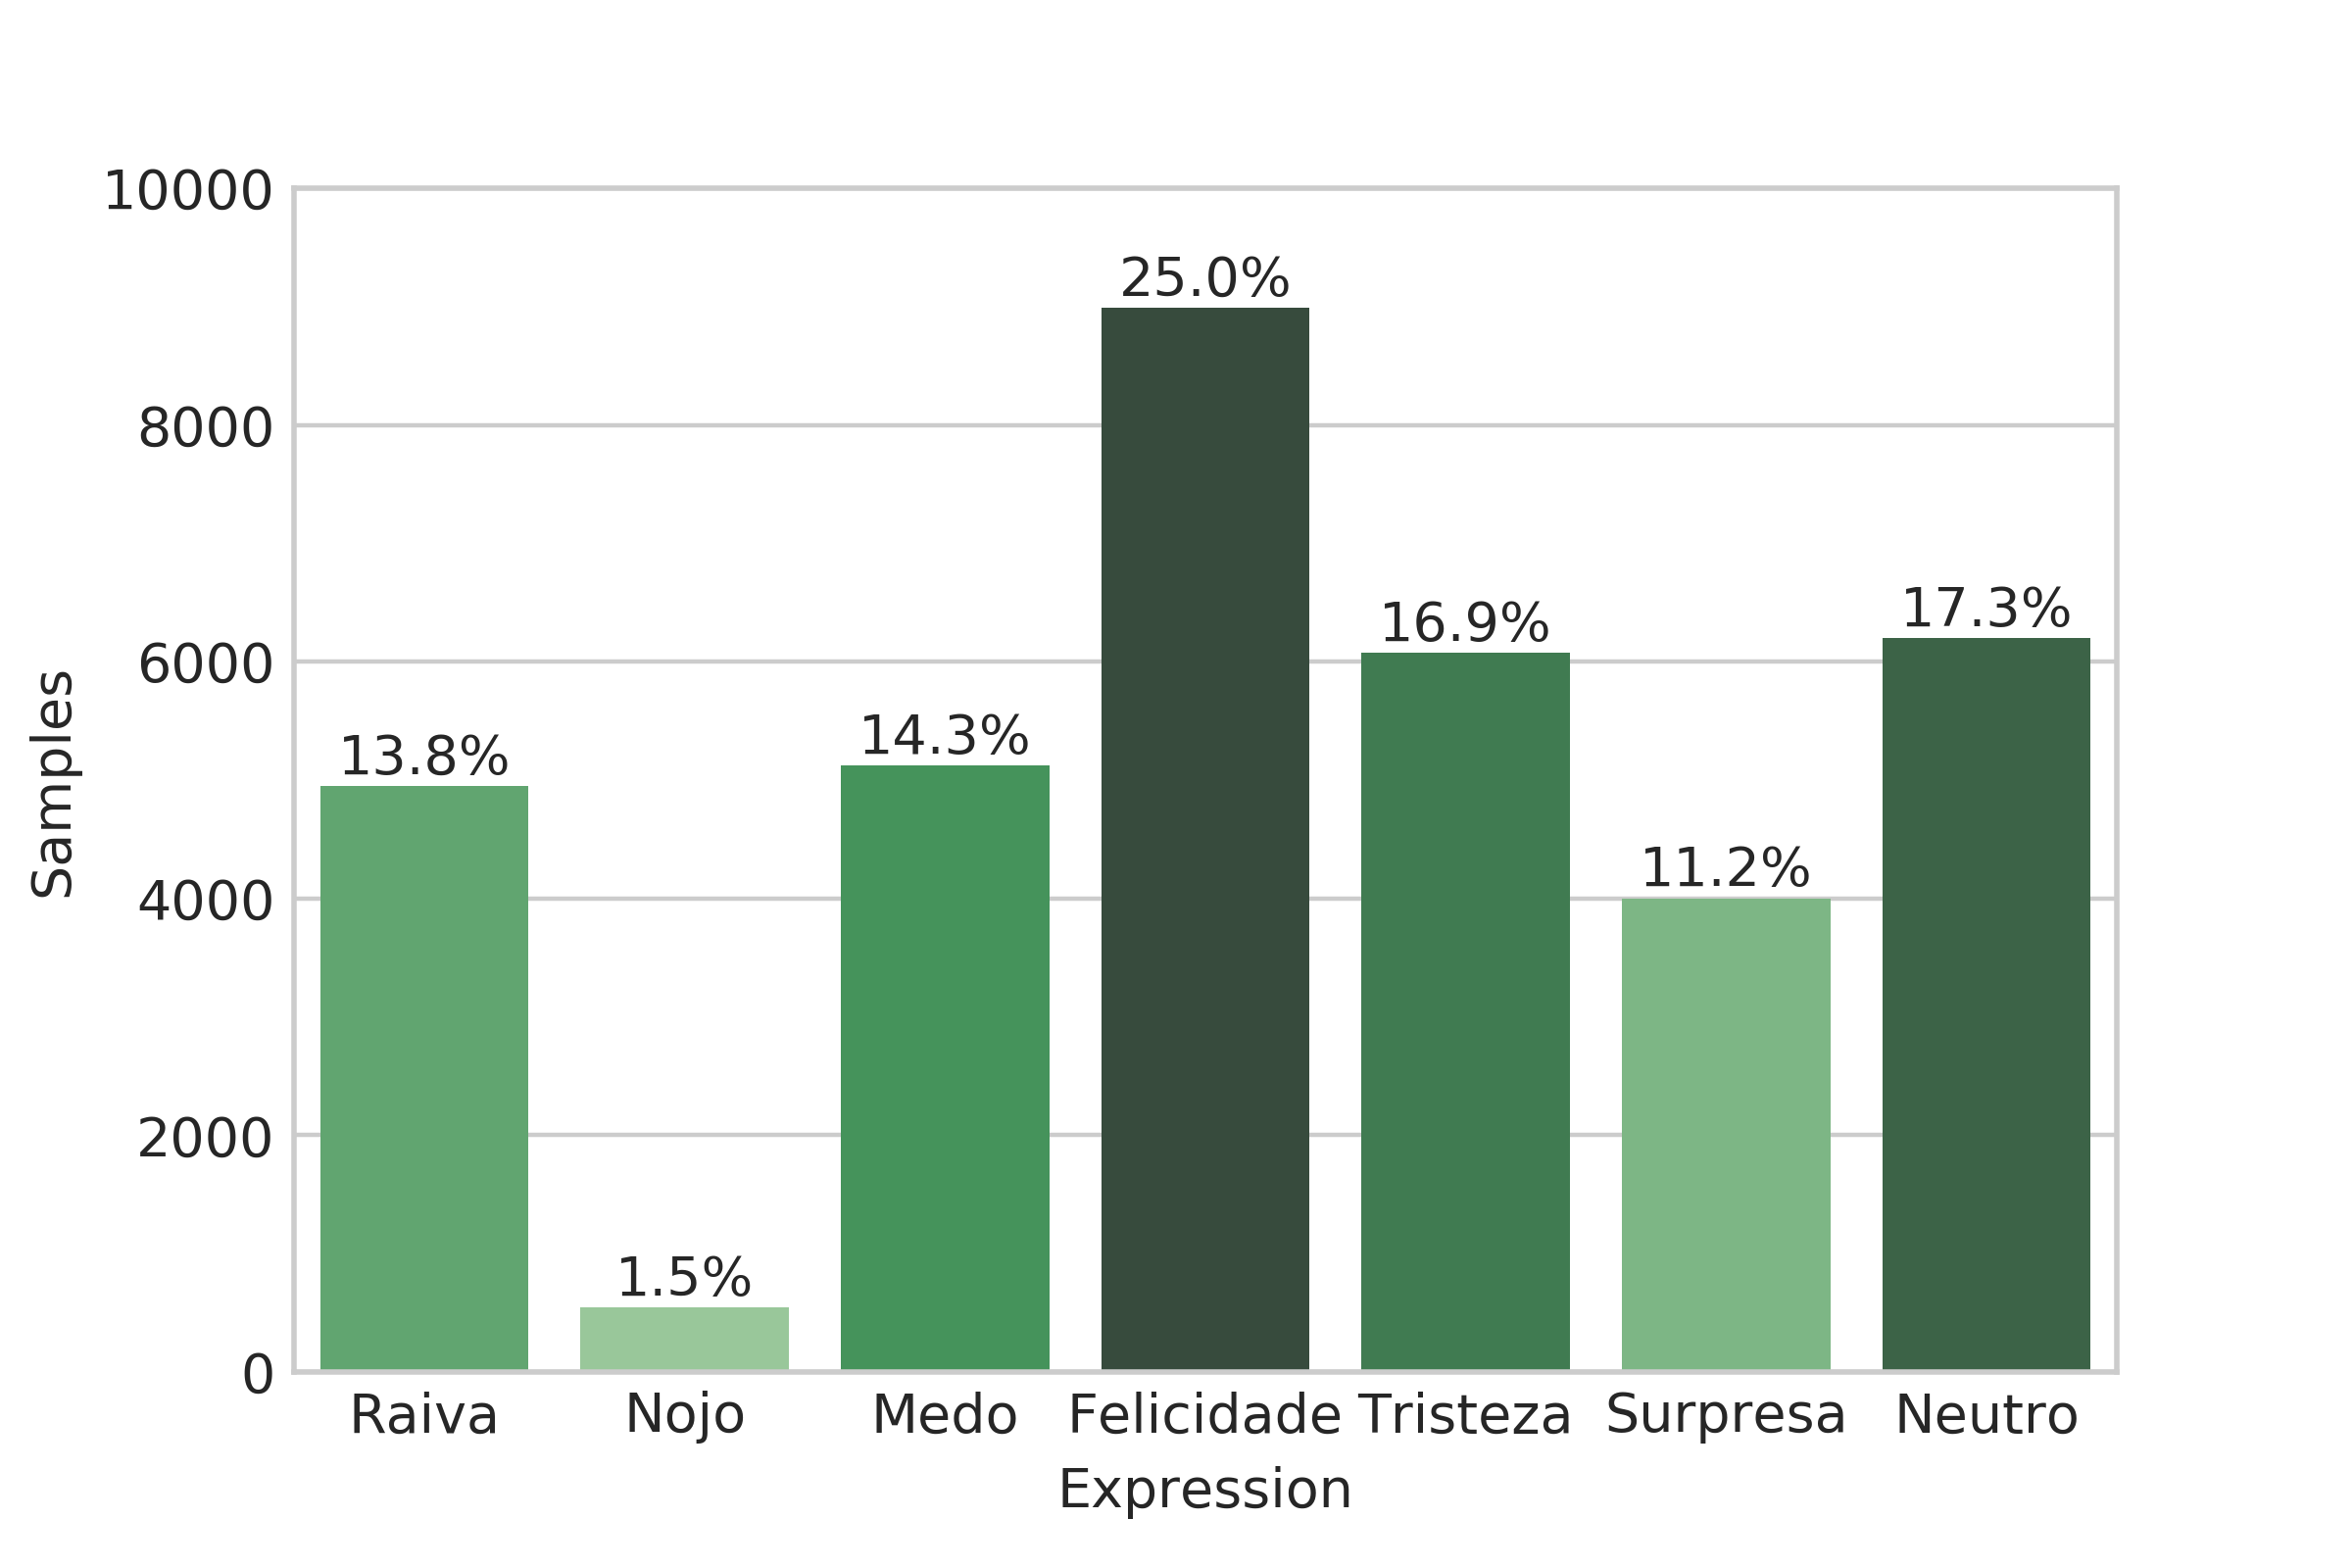
\includegraphics[width=10cm]{images/expression_distribution.png}
\end{figure}

%------------------------------------------------

%------------------------------------------------
\section{Abordagem}
\begin{frame}{Abordagem}
    
\begin{figure}
    \centering
    \begin{small}
    \begin{equation}
        \begin{split}
        \textrm{Input Layer} & \Rightarrow [ (\textrm{Convolution} \rightarrow \textrm{Batch Normalization})\cdot i\\
         &\quad \Rightarrow (\textrm{Pooling} \rightarrow \textrm{Dropout})\cdot j]\cdot k \\
         &\quad \Rightarrow [\textrm{Fully Connected} \rightarrow \textrm{ReLU}]\cdot \ell \\
         &\quad \Rightarrow \textrm{Flatten} \Rightarrow \textrm{Output Layer}
        \end{split}
    \end{equation}
    \end{small}
    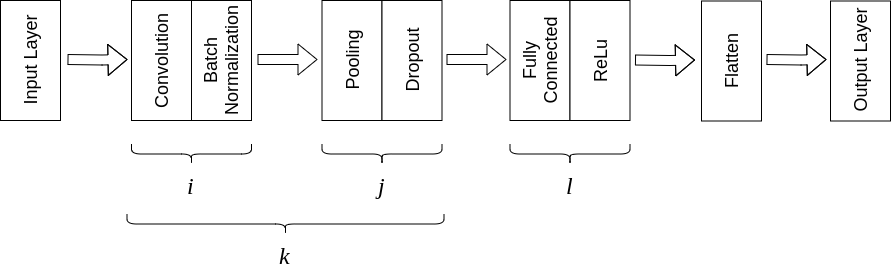
\includegraphics[width=1.0\linewidth]{img/cnn_build.png}
    \caption{Construção de modelos convolucionais.}
\end{figure}
    
\end{frame}
%------------------------------------------------

%------------------------------------------------
\section{Experimentos}
\begin{frame}{Experimentos - K-Fold}

\begin{itemize}
    \item K-Fold
    
      \begin{figure}
    \centering
    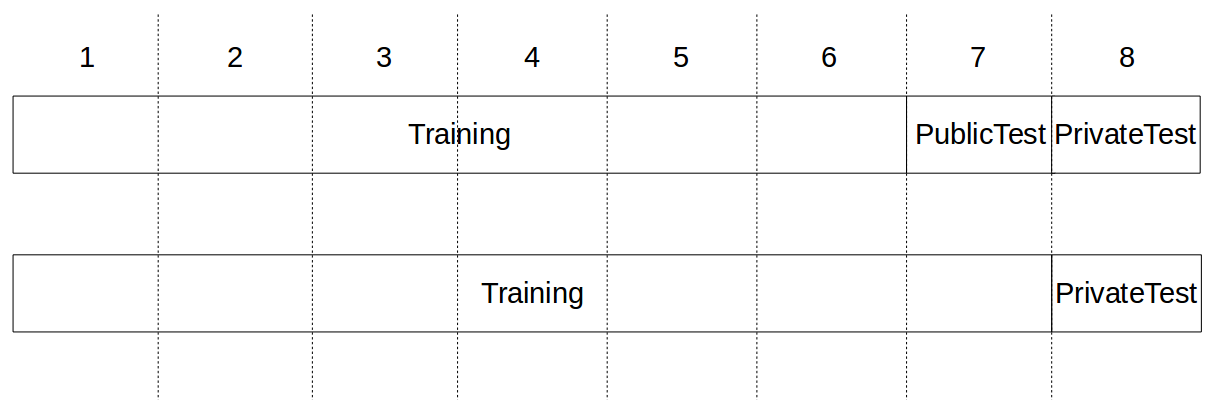
\includegraphics[width=1.0\linewidth]{img/evaluation.png}
    \caption{Divisão de partições do K-Fold.}
  \end{figure}
\end{itemize}

\end{frame}

\begin{frame}{Experimentos - Data augmentation}

    \begin{columns}
    \begin{column}{0.4\textwidth}
      \begin{itemize}
        \item Data augmentation
        \begin{itemize}
            \item Rotação
            \item Translação
            \item Escala
            \item Reflexão
        \end{itemize}
      \end{itemize}
    \end{column}
    
    \begin{column}{0.6\textwidth}
        \begin{figure}
    \centering
    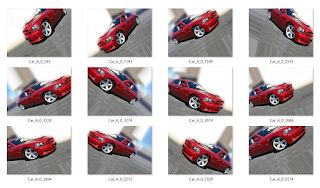
\includegraphics[width=1.0\linewidth]{img/data_augmentation.png}
    \caption{Data augmentation \cite{amaratunga_1970}.}
  \end{figure}
    \end{column}
    
\end{columns} 

\end{frame}

\begin{frame}{Experimentos - Medidas de desempenho}

    \begin{columns}
    \begin{column}{0.3\textwidth}
      \begin{itemize}
        \item Medidas
        \begin{itemize}
            \item F1-Score
            \item Acurácia
        \end{itemize}
      \end{itemize}
    \end{column}
    
    \begin{column}{0.7\textwidth}
        \begin{figure}
    \centering
    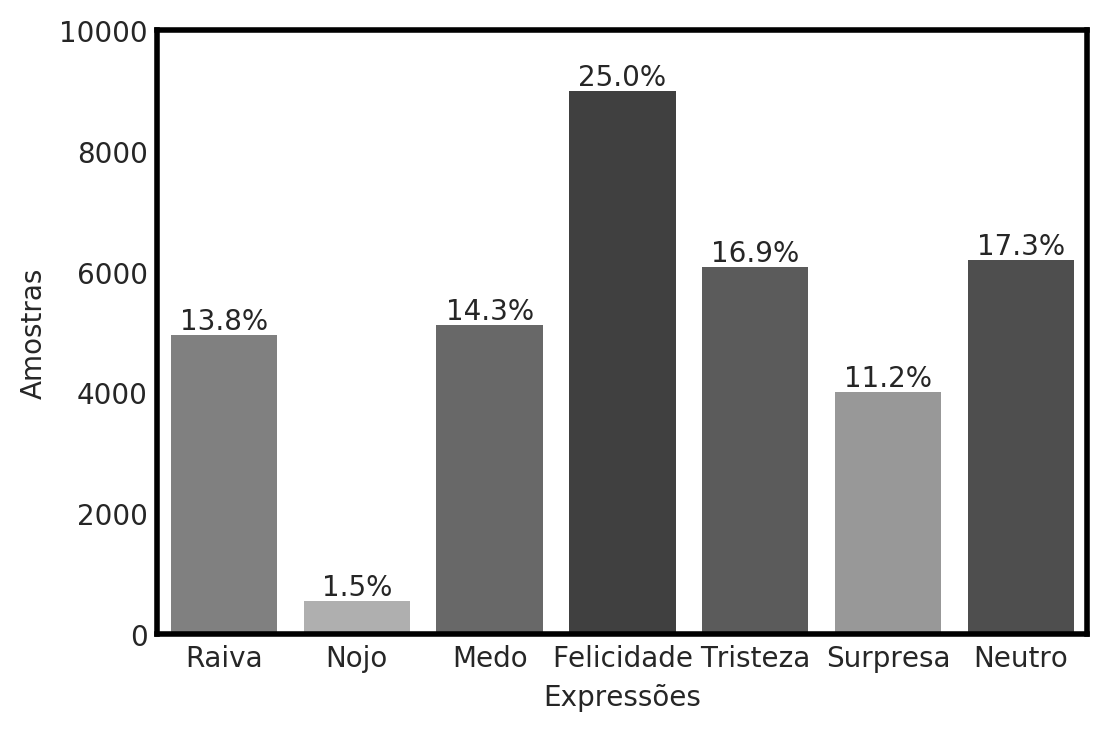
\includegraphics[width=0.9\linewidth]{img/expression_distribution.png}
    \caption{Distribuição de emoções na base de dados.}
  \end{figure}
    \end{column}
    
\end{columns} 

\end{frame}
%------------------------------------------------

%------------------------------------------------
\section{Resultados}
Nesta seção são apresentados os resultados obtidos na metodologia proposta em classificar automaticamente expressões faciais, com base na partição de teste. Em seguida, é analisado o desempenho dos componentes do \textit{Ensemble} na medida Micro \textit{F1 Score}, para cada expressão e por fim  é feita um comparativo com os resultados de trabalhos relacionados. \todo{Citar resultados de trabalhos relacionados}

\subsection{4.1 Classificação das Expressões Faciais}
Para executar a avaliação do modelo proposto na tarefa de classificação, aplicou-se os exemplos contidos na partição de teste, de forma sequencial e supervisionada. Onde o rótulo fornecido pelo modelo para cada exemplo foi armazendo como resultado predito, para futura comparação com o rótulo verdadeiro, que é o contido na base dados.

Após o processo de rotulação das amostras de teste pelo modelo, foram fornecidas as informações de dados rotulados, juntamente dos rótulos verdadeiros, a medida Micro \textit{F1 Score}, onde obteve-se como resultado o valor de $71.74$\%. Contudo, os trabalhos relacionados aqui apresentados fazem uso da medida de acurácia como resultados de desempenho, a qual foi obtida pelo mesmo método da medida Micro \textit{F1 Score}, e resultou em $71.74$\%.


\subsection{4.2 Desempenho dos componentes do \textit{Ensemble}}
O método utilizado para obtenção dos valores de Micro \textit{F1 Score} e acurácia para o \textit{Ensemble} foi o mesmo utilizado para os modelos de Rede Convolucional e \textit{Xtreme Gradient Boosting}. Ressaltando que os resultados das medidas de desempenho obtiveram os mesmos valores, sendo este o motivo de serem apresentados somente o valor da medida Micro \textit{F1 Score}. Na Tabela \ref{tbl:fscore} observa-se os resultados para cada modelo de Rede Convolucional, juntamente do resultado do \textit{Ensemble}.

\begin{table}[!htb]
\centering
\caption{F1 Micro das Arquiteturas utilizadas}
\label{tbl:fscore}
\begin{tabular}{@{}cc@{}}
\toprule
Modelo & F1 Micro           \\ \midrule
1      & 0.6898857620507105 \\
2      & 0.6767901922541097 \\
3      & 0.6606297018668152 \\
4      & 0.6798551128448036 \\
5      & 0.6667595430482028 \\
6      & 0.6781833379771524 \\
7      & 0.694901086653664  \\
8      & 0.6285873502368348 \\
9      & 0.6244079130677069 \\ 
ensemble & 0.7174700473669546 \\ \bottomrule
\end{tabular}
\end{table}

É observado que o melhor classificador, modelo 7, individual de CNN, obteve 69.49\% enquanto que o pior, modelo 9, obteve 62.44\%. Ressaltando que cada classificador de CNN usado no \emph{Ensemble} obteve resultados melhores do que os outros, em determinada expressão ou bons resultados em todas as expressões, mas não se sobressaiu em nenhuma expressão específica. No caso do modelo 9, obteve-se bons resultados em quase todas as expressões, mas nenhum resultado melhor na classificação de determinada expressão em relação aos outros modelos. Já no caso do modelo 7, obteve-se o melhor resultado de classificação para expressão de surpresa.

No modelo \textit{Ensemble} teve-se um total de 32.738.871 parâmetros treináveis, que é resultado da soma dos parâmetros treináveis dos modelos CNN, bem como do XGBoost. Onde o modelo de XGBoost possui uma quantidade pequena de parâmetros treináveis, em comparação com os modelos de CNN, pois, enquanto a quantidade deste está na ordem de milhares, os outros estão na ordem de milhões. Este comportamento se mostra coerente, se for levado em consideração as tarefas de cada modelo, que possuem complexidades bastante distintas.

Os modelos de CNN mais profundos, consequentemente com maior número de parâmetros treináveis, foram os que obtiveram melhores desempenho individuais.   Já os modelos mais rasos, apesar de obterem desempenho abaixo dos profundos, obtiveram os melhores resultados em classificar expressões específicas. Quantidade de parâmetros treináveis do \textit{Ensemble} podem ser visualizados na Tabela \ref{tbl:fscore}.

Na Figura \ref{fig:emsemble} é apresentado o resultado do modelo utilizando \emph{Ensemble}. Onde o resultado final de desempenho foi de 71.74\% de acordo com a métrica \emph{F1 Micro}, ressaltando que seu valor de Acurácia possui o mesmo valor. E com este resultado o \emph{Ensemble} supera, por pouco, o modelo campeão da competição.

\begin{figure}[!htb]
    \centering
    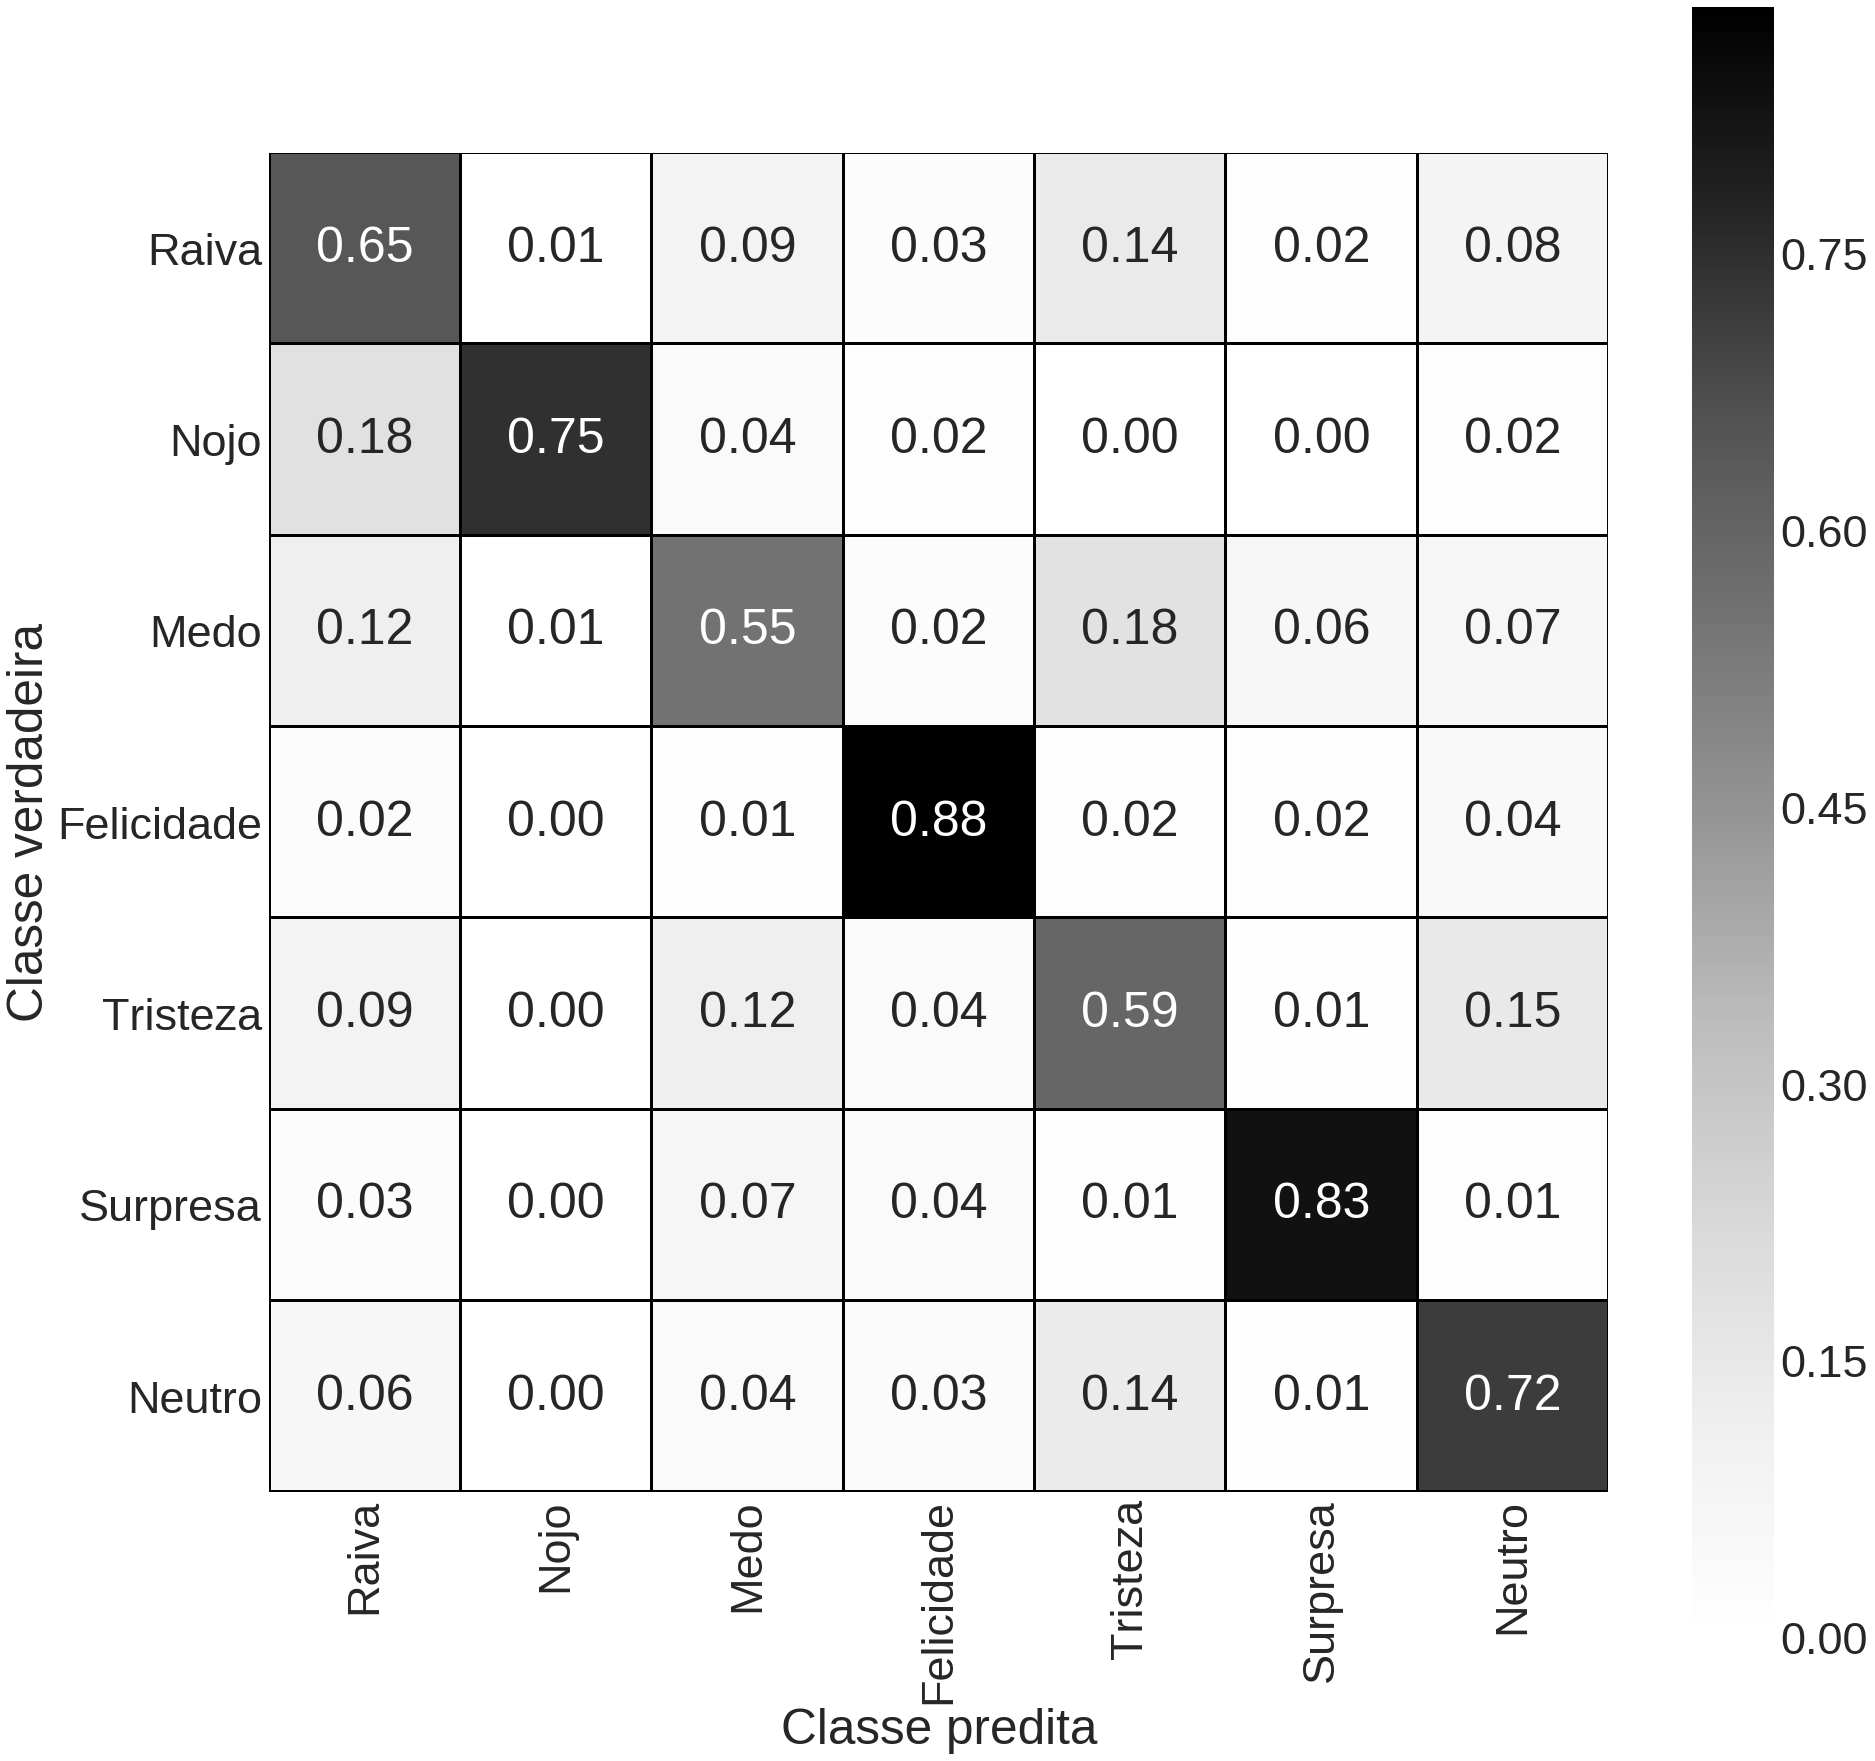
\includegraphics[width=9cm]{images/cm_emsemble.png}
    \caption{Matriz de Confusão do \emph{Ensemble} (CNN + \emph{XGBoost})}
    \label{fig:emsemble}
\end{figure}

Apesar do desbalanceamento da base de dados, a classificação da expressão de nojo obteve-se um dos melhores resultados \ref{fig:samples}, acompanhadas de surpresa e felicidade, com \textit{F1 Score} de
78\%, 83\%, e 89\% respectivamente. As classificações das outras expressões também apresentaram bons resultados, todas com \textit{F1 Score} maior ou igual a 58\%.

\begin{figure}[!htb]
    \centering
    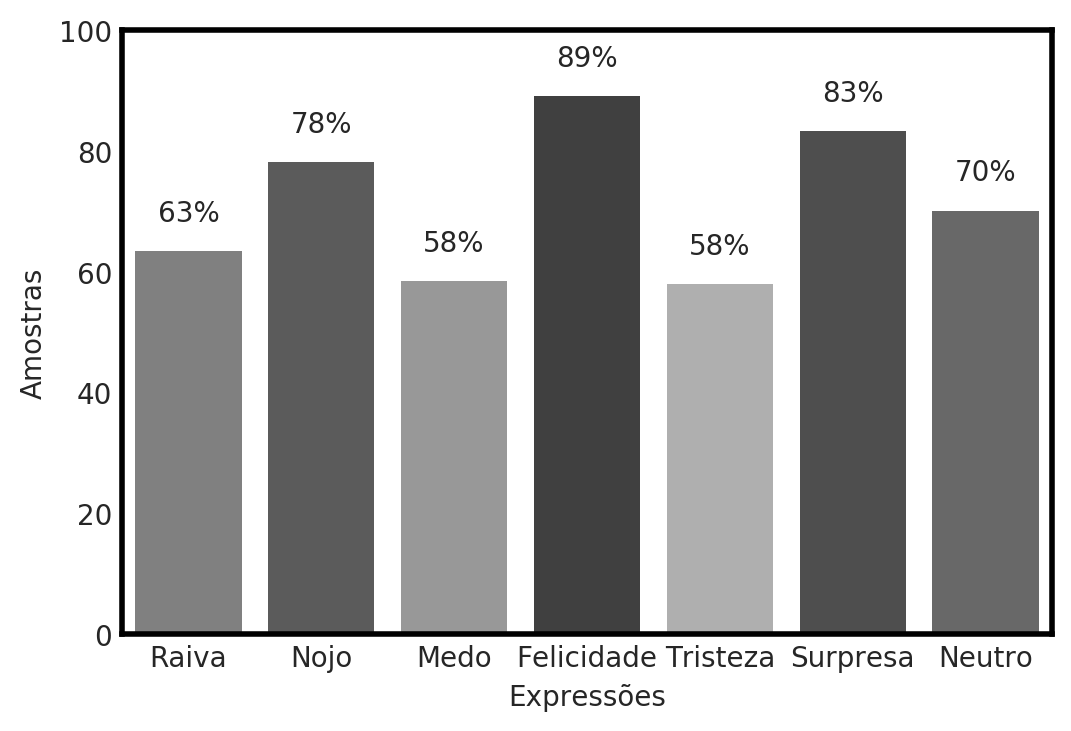
\includegraphics[width=8cm]{images/f1_bar.png}
    \caption{F1 Score por Expressão}
    \label{fig:f1_bar}
\end{figure}


\subsection{4.3 Comparativo de resultados com a literatura}



O modelo proposto conseguiu superar os seres humanos nesta base de dados, na tarefa de classificar as expressões faciais, visto que sua acurácia foi de $71.74$\%, enquanto a dos seres humanos é de $65\pm5$\% \cite{goodfellow2013challenges}.

%------------------------------------------------

%------------------------------------------------
\section{Trabalhos relacionados}
\begin{frame}{Trabalhos relacionados}
    
\begin{table}[!htb]
\centering
\caption{Comparação entre modelo proposto com a literatura}
\label{tbl:results}
\begin{tabular}{@{}cc@{}}
\toprule
Modelo                                                     & Acurácia \\ \midrule
\cite{DBLP:journals/corr/PramerdorferK16} & 75.20     \\
\cite{Kim2016FusingAA}                    & 73.73    \\
\cite{al2016facial}                       & 73.40     \\
\rowcolor{LightCyan} Proposto                                            & 71.74    \\
\cite{DBLP:journals/corr/Tang13}          & 71.20     \\ \bottomrule
\end{tabular}
\end{table}

    
\end{frame}
%------------------------------------------------

%------------------------------------------------
\section{Conclusão}
\section{Conclusão}
Texto
%------------------------------------------------

\section{Referências}
\begin{frame}[allowframebreaks]
\frametitle{Referências}
\bibliographystyle{sbc}
\bibliography{sbc-template}
\end{frame}

% \begin{frame}{Código Fonte}
% \begin{figure}
%     \centering
%     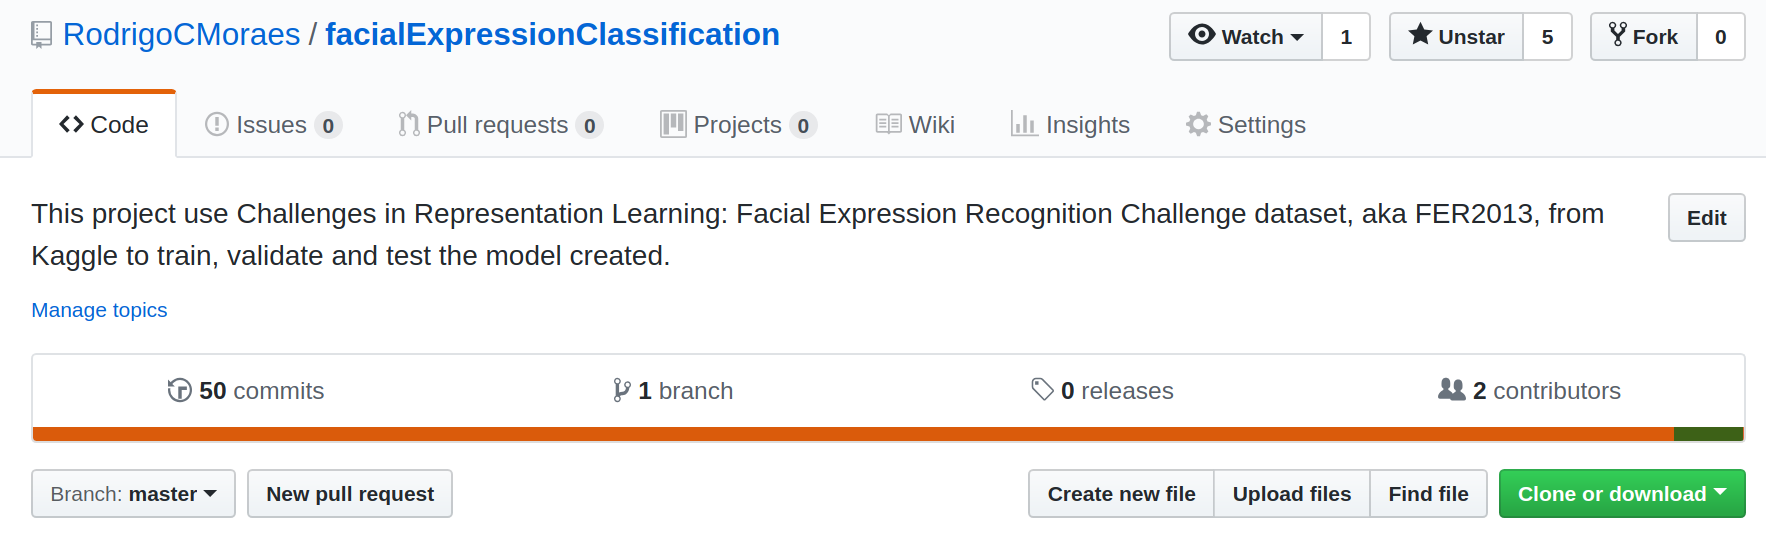
\includegraphics[width=1.0\linewidth]{img/source_code.png}
% \end{figure}
%     \bigskip
%     https://github.com/RodrigoCMoraes/facialExpressionClassification
% \end{frame}

\begin{frame}{Agradecimentos}
    \begin{center}
        \Huge Obrigado
    \end{center}
\end{frame}

\againframe{firstframe}

\end{document}